\documentclass[12pt,letterpaper]{book}
\usepackage[margin=0.7in]{geometry}
\usepackage[utf8]{inputenc} 
\usepackage{graphicx}
\usepackage{amsmath, amsfonts, amssymb, amsthm, thmtools}
\usepackage{braket} 
\usepackage{relsize} 
\usepackage{float}
\usepackage{mathtools}
\usepackage{lmodern} 
\usepackage[T1]{fontenc}
\usepackage{fancyhdr}
\usepackage[dvipsnames]{xcolor} % Colors, use dvipsnames for more color options
\usepackage{framed} % Fancy leftbar
\usepackage[normalem]{ulem}
\usepackage{tikz-cd} % Diagrams
\usepackage{tikz} % General purpose graphics
\usepackage{tikz-3dplot}
\usepackage[most]{tcolorbox} % For theorem boxing
\usepackage{bm} % For better bold math font
\usepackage{old-arrows} 
\usepackage[usestackEOL]{stackengine}
\usepackage[hyperfootnotes=false]{hyperref} % For clickable table of contents
\usepackage{calc} % For simpler calculation - used for spacing the index letter headings correctly
\usepackage{verbatim}
\usepackage{enumitem} % Customize lists
\setitemize{noitemsep,topsep=0.5em, parsep=0.5em ,partopsep=0pt}
\setlist{nolistsep} %  Reduce spacing between bullet points and numbered lists
\usepackage{adjustbox} % Very useful boxing environment
\usepackage{setspace} % Variable line spacing
\linespread{1.1}

%My various environment commands
%%%%%%%%%%%%%%%%%%%%%%%% Theorem Environment %%%%%%%%%%%%%%%%%%%%%%%%
\newenvironment{thm}[1][]{%
  %\ifhmcpset@boxed\def\hmcpset@probenv{boxed}\else\def\hmcpset@probenv{}\fi%
  \bigskip% put space before problem statement box %
  \noindent 

  \begin{tcolorbox}[sharp corners, colback=NavyBlue!2,colframe=blue!70!black!70]% 
    \refstepcounter{theorem}\par\medskip
   \textbf{Theorem \thetheorem. \hspace{-2mm}#1} \rmfamily
  \def\@tempa{#1}%
  \ifx\@tempa\empty\else%
    \hspace{0.5em}%
  \fi%
}{%
  \vspace{0.2cm}
  \end{tcolorbox}%
}

%%%%%%%%%%%%%%%%%%%%%%%%%new Exercise Environment %%%%%%%%%%%%%%%%%%%%%%%%
%Note: if this causes issue in the future, it might be because 
%of the samepage environment. Apparently this environment sucks, but 
%it is used to prevent the top and bottom lines of the exercise 
%enviionment from overlapping on different pages. In those cases, 
%it looks weird, and we always want the statment of an exercise to be
%on the same page.
\newenvironment{exercise}[1][]{
    \begin{samepage}   
    \noindent\rule{\textwidth}{0.5pt}
    \vspace{-10.5mm}
    \def\@tempa{#1}
    \paragraph{#1}
}{
    \hfill\break
    \noindent\rule{\textwidth}{0.5pt}
\end{samepage}
}

%%%%%%%%%%%%%%%%%%%%%%%%% Proof Environment %%%%%%%%%%%%%%%%%%%%%%%%
%leftbar environment for proofs
\newenvironment{proofleftbar}[1][\hsize]
{%
    \def\FrameCommand
    {%
        {\color{black}\vrule width 0.8pt}%
        \hspace{5pt}
        \fboxsep=\FrameSep
    }
    \MakeFramed{\hsize#1\advance\hsize-\width\FrameRestore}%
} 
    {\endMakeFramed}

    \newenvironment{prf}[1][]{%
    \proofleftbar
    \vspace{-.6cm}
    \paragraph{\textit{Proof:}}
}{ 
    {
        \mbox{}\hfill$\blacksquare$
    }
    \endproofleftbar
}

%%%%%%%%%%%%%%%%%%%%%%%%% Variable Proof Environment %%%%%%%%%%%%%%%%%%%%%%%%
\newenvironment{varprf}[1][]{%
    \proofleftbar
    \vspace{-.6cm}
    \paragraph{\textit{#1}}
}{% 
    {%
        \mbox{}\hfill$\blacksquare$
    }
    \endproofleftbar
}

%%%%%%%%%%%%%%%%%%%%%%%%% Remark Environment %%%%%%%%%%%%%%%%%%%%%%%%
%leftbar environment for Remarks. Requires xcolor
\newenvironment{remarkleftbar}[1][\hsize]
{%
    \def\FrameCommand
    {%
        {\color{Plum}\vrule width 0.8pt}%
        \hspace{5pt}
        \fboxsep=\FrameSep%
    }%
    \MakeFramed{\hsize#1\advance\hsize-\width\FrameRestore}%
}
{\endMakeFramed}

\newenvironment{remark}[1][]{%
    \remarkleftbar
    \vspace{-.6cm}
    \addtocounter{theorem}{1}
    \paragraph{\textbf{Remark \thetheorem.}}
}
{ 
    \endremarkleftbar
}


%%%%%%%%%%%%%%%%%%%%%%%% Solution Environment %%%%%%%%%%%%%%%%%%%%%%%%

\newenvironment{solution}[1][]{{
    \noindent\textit{\textbf{Solution:}}}
    }{ 
        {
            \mbox{}\hfill$\blacksquare$
        }
    }

%%%%%%%%%%%%%%%%%%%%%%%%% Example Environment %%%%%%%%%%%%%%%%%%%%%%%%
\newenvironment{example}[1][]{
    {\begin{minipage}{\textwidth}
        \begin{center}
            \rule{8cm}{0.4pt}
        \end{center}
    \end{minipage}
    \addtocounter{theorem}{1}
    \textbf{Example \thetheorem.}
  }
 }{
    \vskip0pt
    \begin{minipage}{\textwidth}
        \begin{center}
            \rule{8cm}{0.4pt}
        \end{center}
    \end{minipage}
  }

%%%%%%%%%%%%%%%%%%%%%%%% Important Statement Environment %%%%%%%%%%%%%%%%%%%%%%%%
\newenvironment{statementleftbar}[2][\hsize]
{%
    \def\FrameCommand
    {%
        {\color{black}\vrule width 2.5pt}%
        \hspace{0pt}%must no space.
        \fboxsep=\FrameSep\colorbox{#2}%
    }%
    \MakeFramed{\hsize#1\advance\hsize-\width\FrameRestore}%
}{
  \endMakeFramed
  }

\newenvironment{statement}[1]{%
\statementleftbar{#1}
}{ 
  \endstatementleftbar
}
%%%%%%%%%%%%%%%%%%%%%%%% Align environment, no space %%%%%%%%%%%%%%%%%%%%%%%%
%sometimes the AMS math environment align's extra vertical space on the 
%top and bottom is super annoying when one uses align in a special box 
%or something. This is a solution.

%%%% Removes top and bottom space. 
\newenvironment{align_topbot}[1][]{

  \centering
  $\begin{aligned}
}
{
  \end{aligned}$
  \par
}

%%%% Removes bottom space, leaves top space. 
%%%% This is what you probably 
%%%% want, and this is mostly used when a boxed environment or something 
%%%% ENDS with an equation, and you don't want to waste extra space at the bottom.
\newenvironment{align_top}[1][]{
  \vspace{0.4cm}
  \centering
  $\begin{aligned}
}
{
  \end{aligned}$
  \par
}
%%%% Leaves bottom space, removes top space. Probably won't ever use this. 
\newenvironment{align_bot}[1][]{
  \centering
  $\begin{aligned}
}
{
  \end{aligned}$
  \par
  \vspace{0.4cm}
}
%%%%% Of course, if you want both spaces, just use align from AMS.

 

% All images lie in pictures folder
\graphicspath{{pictures/}}

% For clickable table of contents
\hypersetup{ 
    colorlinks,
    citecolor=black,
    filecolor=black,
    linkcolor=black,
    urlcolor=black
}
\usetikzlibrary{arrows, 
arrows.meta, 
braids, 
calc, 
shapes.geometric,
arrows,
decorations.markings,
decorations.pathreplacing, 
intersections,
hobby
}
% Tikzcd specifications
\tikzcdset{arrow style = tikz, diagrams={>={Stealth[scale=0.75]}}} % Use stealth arrows in CDs
\tikzset{>={Stealth[scale=1]}} % Use stealth arrows in TiKZ graphics
\newcommand{\smallish}{1.45em} % Unit for measuring

% Better \to command
\renewcommand{\to}{\mathbin{\tikz[baseline] \draw[-{Stealth[length=5pt,width=4pt]}] (0pt,.6ex) -- (3.5ex,.6ex);}}

% Barrage of shorcuts
\newcommand{\normal}{\unlhd}
\newcommand{\im}{\mbox{Im}}
\newcommand{\nat}{\mbox{Nat}}
\newcommand{\ZZ}{\mathbb{Z}}
\newcommand{\RR}{\mathbb{R}}
\newcommand{\NN}{\mathbb{N}}
\newcommand{\zz}{\mathbb{Z}}
\newcommand{\rr}{\mathbb{R}}
\newcommand{\nn}{\mathbb{N}}
\newcommand{\qq}{\mathbb{Q}}
\renewcommand{\phi}{\varphi}

% Theorem customization and colorings
\theoremstyle{definition}
\newtheorem{theorem}{Theorem}[section]

\declaretheoremstyle[
    spacebelow=6pt,%
    headfont=\color{RoyalPurple}\normalfont\bfseries,
]{colors}

\declaretheorem[
  style=colors,
  name=Definition,
  sibling=theorem
]{definition}

\declaretheoremstyle[
    spacebelow=6pt,%
    headfont=\color{RoyalBlue}\normalfont\bfseries,
]{colorss}

\declaretheorem[
  sibling=theorem,
  style=colorss,
  name=Proposition,
]{proposition}

\declaretheoremstyle[
    spacebelow=6pt,%
    headfont=\color{RoyalBlue}\normalfont\bfseries,
]{colorsss}

\declaretheorem[ 
  style=colorsss,
  name=Corollary,
  sibling=theorem
]{corollary}

\declaretheoremstyle[
    spacebelow=6pt,%
    headfont=\color{RoyalBlue}\normalfont\bfseries,
]{colorssss}

\declaretheorem[
  style=colorssss,
  name=Lemma,
  sibling=theorem
]{lemma}

\renewcommand{\contentsname}{}

\begin{document} 
  \chapter{Introduction}
  \section{Neural Networks}
  Neural networks represent a mathematical tool in machine learning that is useful for performing function 
  approximation; they can be thought of as a generalization of linear regression. The power of a neural network stems 
  from three main properties that we will go over: nonliterary, differentiability, and hidden layers.
  These key properties allow neural networks to be able to improve its approximation of a set of values via ``training.'' 

  To kick things off we will start with a simple example of a neural network.
  In the simplest form, a neural network consists of a \textbf{vector input} $\vec{x} \in \mathbb{R}^n$, a set 
  of \textbf{weights} $w_i \in \mathbb{R}$, and a final \textbf{output} $y \in \mathbb{R}$.
  Below is a graphical representation of a such network. 
  \begin{center}
  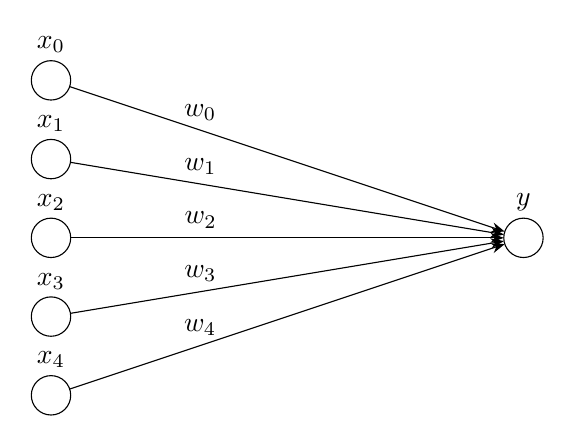
\begin{tikzpicture}
    \draw[->] (0.23717082451262844, 3.9209430584957907) to (5.762829175487371, 2.0790569415042093);
    \draw (0, 4) circle (0.25cm);
    \node at (0, 4.45) { $x_0$ };
    \node[above] at (1.8948683298050513, 3.368377223398316) { $w_0$ };
    \draw[->] (0.24659848095803594, 2.9589002531736606) to (5.753401519041964, 2.0410997468263394);
    \draw (0, 3) circle (0.25cm);
    \node at (0, 3.45) { $x_1$ };
    \node[above] at (1.8986393923832146, 2.683560101269464) { $w_1$ };
    \draw[->] (0.25, 2.0) to (5.75, 2.0);
    \draw (0, 2) circle (0.25cm);
    \node at (0, 2.45) { $x_2$ };
    \node[above] at (1.9, 2.0) { $w_2$ };
    \draw[->] (0.24659848095803594, 1.0410997468263392) to (5.753401519041964, 1.9589002531736608);
    \draw (0, 1) circle (0.25cm);
    \node at (0, 1.45) { $x_3$ };
    \node[above] at (1.8986393923832146, 1.3164398987305357) { $w_3$ };
    \draw[->] (0.23717082451262844, 0.07905694150420949) to (5.762829175487371, 1.9209430584957905);
    \draw (0, 0) circle (0.25cm);
    \node at (0, 0.45) { $x_4$ };
    \node[above] at (1.8948683298050513, 0.6316227766016838) { $w_4$ };
    \draw (6, 2) circle (0.25cm);
    \node at (6, 2.45) { $y$ };
  \end{tikzpicture}
  \end{center}
  In such a graphical representation, the set of $x_i$ nodes are called the \textbf{input layer} (or simply the first layer)
  and the $y$ node is called the \textbf{output layer}. In the above diagram, the output layer 
  consists of one node, but as we will see it can also consist of multiple nodes.

  The output is obtained as a function of the input and weights as below.
  \[
    y = \sum_{i} w_ix_i  
  \] 
  From a statistics perspective, this is actually just a \textbf{linear model}. In statistics, 
  one ``trains'' such a linear model via linear regression on some dataset. If you have 
  taken a statistics course, you might remember that this strategy works on simple 
  examples (e.g., a suspiciously-already-linear weather dataset in a Pearson textbook), 
  but linear models do not generalize and often fail to capture complex behavior.

  As we will see, neural networks are different from linear models since they add properties 
  of hidden layers and nonlinearity.
  
  \section{Hidden Layers}

  Neural networks extend our previous notion of a linear model via \textbf{hidden layers}, which can 
  be defined as one or more layers between the input and output layer. Below, we have 
  a neural network which has one hidden layer. The hidden layer can 
  have a variable number of nodes, but in our example below we have five.

  In this example, each input node $x_i$ connects to each node $h_j$ in the hidden layer 
  via a weight $w_{ij}$. These weights are illustrated by the arrows, although we are 
  choosing to suppress the $w_{ij}$ notation in the diagram below to not over complicate the figure.  
  \begin{center}
    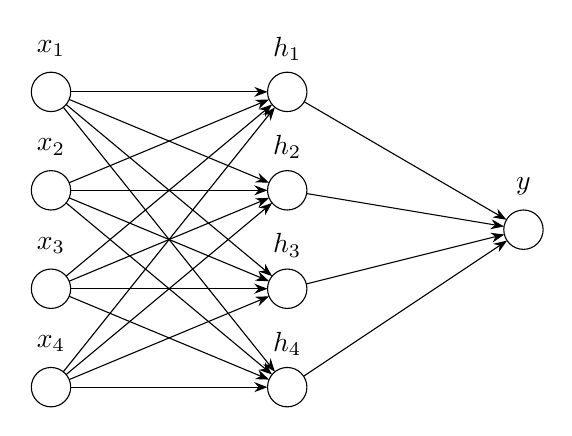
\begin{tikzpicture}
      \draw (0, 3.75) circle (0.25cm);
      \node at (0, 4.3) { $x_1$ };
      \draw (0, 2.5) circle (0.25cm);
      \node at (0, 3.05) { $x_2$ };
      \draw (0, 1.25) circle (0.25cm);
      \node at (0, 1.8) { $x_3$ };
      \draw (0, 0.0) circle (0.25cm);
      \node at (0, 0.55) { $x_4$ };
      \draw (3, 3.75) circle (0.25cm);
      \node at (3, 4.3) { $h_1$ };
      \draw (3, 2.5) circle (0.25cm);
      \node at (3, 3.05) { $h_2$ };
      \draw (3, 1.25) circle (0.25cm);
      \node at (3, 1.8) { $h_3$ };
      \draw (3, 0.0) circle (0.25cm);
      \node at (3, 0.55) { $h_4$ };
      \draw (6, 2) circle (0.25cm);
      \node at (6, 2.55) { $y$ };
      \draw[->] (0.25, 3.75) to (2.75, 3.75);
      \draw[->] (0.23076923076923075, 3.6538461538461537) to (2.769230769230769, 2.5961538461538463);
      \draw[->] (0.19205531989934396, 3.58995390008388) to (2.8079446801006562, 1.41004609991612);
      \draw[->] (0.15617376188860607, 3.5547827976392425) to (2.843826238111394, 0.19521720236075757);
      \draw[->] (0.23076923076923075, 2.5961538461538463) to (2.769230769230769, 3.6538461538461537);
      \draw[->] (0.25, 2.5) to (2.75, 2.5);
      \draw[->] (0.23076923076923075, 2.4038461538461537) to (2.769230769230769, 1.3461538461538463);
      \draw[->] (0.19205531989934396, 2.33995390008388) to (2.8079446801006562, 0.16004609991611995);
      \draw[->] (0.19205531989934396, 1.41004609991612) to (2.8079446801006562, 3.58995390008388);
      \draw[->] (0.23076923076923075, 1.3461538461538463) to (2.769230769230769, 2.4038461538461537);
      \draw[->] (0.25, 1.25) to (2.75, 1.25);
      \draw[->] (0.23076923076923075, 1.1538461538461537) to (2.769230769230769, 0.09615384615384617);
      \draw[->] (0.15617376188860607, 0.19521720236075757) to (2.843826238111394, 3.5547827976392425);
      \draw[->] (0.19205531989934396, 0.16004609991611995) to (2.8079446801006562, 2.33995390008388);
      \draw[->] (0.23076923076923075, 0.09615384615384617) to (2.769230769230769, 1.1538461538461537);
      \draw[->] (0.25, -1.5308084989341915e-17) to (2.75, 1.5308084989341915e-17);
      \draw[->] (3.2159447252246083, 3.6240322436189785) to (5.784055274775391, 2.1259677563810215);
      \draw[->] (3.2465984809580357, 2.4589002531736606) to (5.753401519041964, 2.0410997468263394);
      \draw[->] (3.242535625036333, 1.3106339062590833) to (5.757464374963667, 1.9393660937409167);
      \draw[->] (3.208012573584461, 0.1386750490563073) to (5.791987426415539, 1.8613249509436927);
    \end{tikzpicture}
  \end{center}
  The calculation of a hidden layer is simply 
  \[
      h_i = \sum_{j}w_{ij}x_j
  \]  
  Intuitively, this means that each input value $x_i$ makes a weighted contribution of $w_{ij}$ 
  to the value $h_j$. Something to observe at this point is that we can summarize the entire hidden layer 
  calculation as a matrix equation:
  \begin{align}
    \vec{h}=
    \begin{bmatrix}
      h_{1} \\
      h_{2} \\
      h_{3} \\
      h_{4} \\
    \end{bmatrix}
    = \begin{bmatrix}
      \sum_{i}w_{1i}x_i \\
      \sum_{i}w_{2i}x_i \\
      \sum_{i}w_{3i}x_i \\
      \sum_{i}w_{4i}x_i \\
    \end{bmatrix}
    = \begin{bmatrix}
      w_{11} & w_{12} & w_{13} & w_{14}\\
      w_{21} & w_{22} & w_{23} & w_{24}\\
      w_{31} & w_{32} & w_{33} & w_{34}\\
      w_{41} & w_{42} & w_{43} & w_{44}\\
    \end{bmatrix}
    \cdot
    \begin{bmatrix}
      x_{1} \\
      x_{2} \\
      x_{3} \\
      x_{4} \\
    \end{bmatrix}
    = 
    W\vec{x}
  \end{align}
  This suggest the concept of a \textbf{weight matrix} $W$, which is the key to calculating the 
  hidden layer $\vec{h}$ from the input $\vec{x}$. For a neural network that has 
  multiple hidden layers, there are multiple corresponding weight matrices. In fact, 
  a neural network with $N$ layers will have $(N-1)$-many weight matrices. 

  For our current example, we will let $U$ denote the matrix of 
  the weights between the output layer and the hidden layer, so that 
  $y = U\vec{h}$. 

  Often times with neural networks it is necessary to introduce a \textbf{bias} in each layer.   
  A bias is an extra node, assigned a value of 1, that we can add to a layer 
  which will be used to contribute to the calculation of the next layer. Below we illustrate the network 
  we'd obtain by adding bias to our previous network.

  \begin{center}
    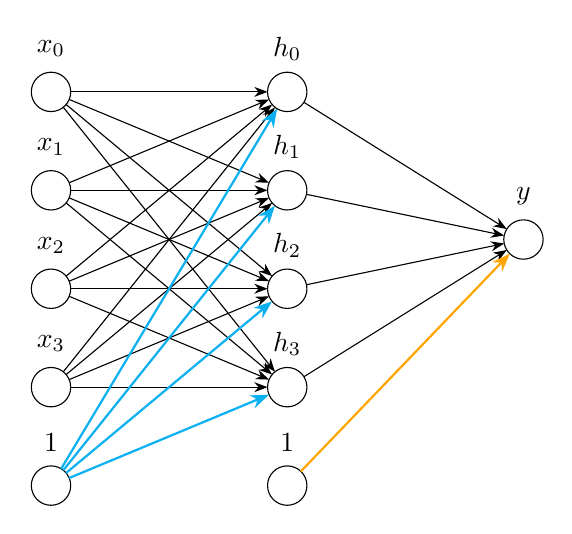
\begin{tikzpicture}
      \draw (0, 5.0) circle (0.25cm);
      \node at (0, 5.55) { $x_0$ };
      \draw (0, 3.75) circle (0.25cm);
      \node at (0, 4.3) { $x_1$ };
      \draw (0, 2.5) circle (0.25cm);
      \node at (0, 3.05) { $x_2$ };
      \draw (0, 1.25) circle (0.25cm);
      \node at (0, 1.8) { $x_3$ };
      \draw (0, 0.0) circle (0.25cm);
      \node at (0, 0.55) { $1$ };
      \draw (3, 5.0) circle (0.25cm);
      \node at (3, 5.55) { $h_0$ };
      \draw (3, 3.75) circle (0.25cm);
      \node at (3, 4.3) { $h_1$ };
      \draw (3, 2.5) circle (0.25cm);
      \node at (3, 3.05) { $h_2$ };
      \draw (3, 1.25) circle (0.25cm);
      \node at (3, 1.8) { $h_3$ };
      \draw (3, 0.0) circle (0.25cm);
      \node at (3, 0.55) { $1$ };
      \draw (6, 3.125) circle (0.25cm);
      \node at (6, 3.675) { $y$ };
      \draw[->, ] (0.25, 5.0) to (2.75, 5.0);
      \draw[->, ] (0.23076923076923075, 4.903846153846154) to (2.769230769230769, 3.8461538461538463);
      \draw[->, ] (0.19205531989934396, 4.83995390008388) to (2.8079446801006562, 2.66004609991612);
      \draw[->, ] (0.15617376188860607, 4.804782797639242) to (2.843826238111394, 1.4452172023607575);
      \draw[->, ] (0.23076923076923075, 3.8461538461538463) to (2.769230769230769, 4.903846153846154);
      \draw[->, ] (0.25, 3.75) to (2.75, 3.75);
      \draw[->, ] (0.23076923076923075, 3.6538461538461537) to (2.769230769230769, 2.5961538461538463);
      \draw[->, ] (0.19205531989934396, 3.58995390008388) to (2.8079446801006562, 1.41004609991612);
      \draw[->, ] (0.19205531989934396, 2.66004609991612) to (2.8079446801006562, 4.83995390008388);
      \draw[->, ] (0.23076923076923075, 2.5961538461538463) to (2.769230769230769, 3.6538461538461537);
      \draw[->, ] (0.25, 2.5) to (2.75, 2.5);
      \draw[->, ] (0.23076923076923075, 2.4038461538461537) to (2.769230769230769, 1.3461538461538463);
      \draw[->, ] (0.15617376188860607, 1.4452172023607575) to (2.843826238111394, 4.804782797639242);
      \draw[->, ] (0.19205531989934396, 1.41004609991612) to (2.8079446801006562, 3.58995390008388);
      \draw[->, ] (0.23076923076923075, 1.3461538461538463) to (2.769230769230769, 2.4038461538461537);
      \draw[->, ] (0.25, 1.25) to (2.75, 1.25);
      \draw[->, color=ProcessBlue, thick] (0.12862393885688164, 0.21437323142813605) to (2.8713760611431183, 4.785626768571864);
      \draw[->, color=ProcessBlue, thick] (0.15617376188860607, 0.19521720236075757) to (2.843826238111394, 3.5547827976392425);
      \draw[->, color=ProcessBlue, thick] (0.19205531989934396, 0.16004609991611995) to (2.8079446801006562, 2.33995390008388);
      \draw[->, color=ProcessBlue, thick] (0.23076923076923075, 0.09615384615384617) to (2.769230769230769, 1.1538461538461537);
      \draw[->, ] (3.211999576001272, 4.867500264999205) to (5.788000423998728, 3.257499735000795);
      \draw[->, ] (3.244745104934401, 3.699011436472) to (5.755254895065598, 3.175988563528);
      \draw[->, ] (3.244745104934401, 2.550988563528) to (5.755254895065598, 3.074011436472);
      \draw[->, ] (3.211999576001272, 1.382499735000795) to (5.788000423998728, 2.992500264999205);
      \draw[->, color=Orange, thick] (3.1731329570474283, 0.18034683025773787) to (5.826867042952571, 2.944653169742262);
    \end{tikzpicture}
  \end{center}
  With this neural network architecture, we have the following weight matrices:
  \[
    W = \begin{bmatrix}
      w_{11} & w_{12} & w_{13} & w_{14} & \textcolor{ProcessBlue}{w_{15}} \\
      w_{21} & w_{22} & w_{23} & w_{24} & \textcolor{ProcessBlue}{w_{25}}\\
      w_{31} & w_{32} & w_{33} & w_{34} & \textcolor{ProcessBlue}{w_{35}}\\
      w_{41} & w_{42} & w_{43} & w_{44} & \textcolor{ProcessBlue}{w_{45}}\\
    \end{bmatrix}
    \hspace{1cm}
    U = \begin{bmatrix}
      u_{11} & u_{12} & u_{13} & u_{14} & \textcolor{Orange}{w_{15}} \\
    \end{bmatrix}
  \]
  Thus, adding a bias to a layer is equivalent to adding a new column to the weight matrix. 
  Our input $[x_1, x_2, x_3, x_4]$ is still in $\mathbb{R}^4$, but we now instead 
  feed the neural network a value of $[x_1, x_2, x_3, x_4, 1]^T \in \mathbb{R}^5.$

  However, note that we're not really doing much mathematically by adding a hidden layer. 
  Observe that we can rewrite $y$ as 
  \[
      y = U\vec{h} = U(W\vec{x}) = W'\vec{x} 
  \]
  where $W' = UW$. This reduces our above network, with three layers, to a boring network, with two layers (similar to the one 
  we started with), just with a different weight matrix $W'$. 
  The reason is because our network is linear, which means 
  no matter how many layers we add it will always reduce to the same boring network we started with. 
  As we know, linear patterns cannot adequately capture complex patterns.
  Thus in order to get something interesting with hidden layers we need to add some nonlinearity.
  
  \section{Nonlinearity}
  Neural networks achieve our desired property of nonlinearity via usage of \textbf{activation fuctions}.
  An activation function is a function $f$ that is called on the summation of a given node in a network, allowing 
  us to modify the calculation for a node $h_i$ as below.
  \[
    h_i = f\left(\sum_{j}w_{ij}x_j\right)
  \]
  We can introduce nonlinearity into our system if we design $f$ to be nonlinear. 

  A few common examples of such functions are the sigmoid (also known as logistic), tanh or RELU functions.
  The machine learning community has gone through several iterations of what is considered to be 
  best practice for an activation function. In the 1990s, the sigmoid function was used very widely.
  In the later 90s and early 2000s, it was discovered that the tanh function lead to be better 
  training performance. Later, it was the discovered that the ReLU function lead to even better 
  training performance. As a result, most modern neural networks will use this for the 
  activation function. 

  Let's introduce the activation functions we just discussed. Below, we have 
  the sigmoid function
  \[
      \sigma(x) = \frac{1}{1 + e^{-x}}
  \]
  and the graph of the sigmoid function is given below.
  \begin{center}
    \begin{tikzpicture}
      \begin{scope}
    \draw[Gray!30, ->] (-4, 0) to (4, 0);
    \draw[Gray!30, ->] (0, 0) to (0, 5.0);
    \node[below] at (4, 0) { $x$ };
    \node[left] at (0, 5.0) { $y$ };
  \end{scope}
  
      \draw[dashed] (-3.5, 4.5) to (4.5, 4.5);
      \draw[fill] (0, 4.5) circle (0.01cm);
      \node[left] at (-3.5, 4.5) { $y=1$ };
      \draw[ProcessBlue] plot coordinates {(-4.5, 0.005262796192749818) (-4.454773869346734, 0.005631746396210898) (-4.409547738693467, 0.006026527305014147) (-4.364321608040201, 0.006448942330119109) (-4.319095477386934, 0.006900920060491525) (-4.273869346733669, 0.0073845228460029805) (-4.228643216080402, 0.007901955953416093) (-4.183417085427136, 0.008455577331464884) (-4.138190954773869, 0.009047908022967094) (-4.092964824120603, 0.009681643263881561) (-4.047738693467337, 0.01035966431124376) (-4.00251256281407, 0.011085051043962974) (-3.9572864321608043, 0.011861095382535868) (-3.9120603015075375, 0.01269131557580394) (-3.866834170854271, 0.013579471404940771) (-3.821608040201005, 0.014529580356873897) (-3.776381909547739, 0.015545934821298967) (-3.7311557788944727, 0.01663312036729784) (-3.685929648241206, 0.017796035157289784) (-3.64070351758794, 0.019039910557579216) (-3.5954773869346734, 0.020370333006064664) (-3.550251256281407, 0.02179326719867715) (-3.505025125628141, 0.02331508065675532) (-3.459798994974874, 0.024942569737754265) (-3.414572864321608, 0.026682987151332882) (-3.369346733668342, 0.0285440710418642) (-3.324120603015076, 0.030534075696637793) (-3.2788944723618094, 0.032661803936339655) (-3.2336683417085426, 0.03493664124063683) (-3.1884422110552766, 0.037368591656690056) (-3.14321608040201, 0.03996831553195919) (-3.0979899497487438, 0.04274716910453138) (-3.052763819095478, 0.0457172459741365) (-3.007537688442211, 0.04889142046473615) (-2.9623115577889445, 0.05228339287476804) (-2.9170854271356785, 0.05590773659345733) (-2.871859296482412, 0.059779947040685594) (-2.8266331658291457, 0.06391649236333043) (-2.7814070351758797, 0.06833486579230547) (-2.7361809045226133, 0.07305363953125817) (-2.690954773869347, 0.07809252000951472) (-2.6457286432160805, 0.0834724042878502) (-2.600502512562814, 0.08921543735544614) (-2.555276381909548, 0.09534506999939227) (-2.5100502512562812, 0.10188611686370903) (-2.4648241206030153, 0.10886481424252653) (-2.419597989949749, 0.11630887707120185) (-2.3743718592964824, 0.12424755448927133) (-2.329145728643216, 0.13271168324978544) (-2.28391959798995, 0.1417337381404277) (-2.2386934673366836, 0.15134787846268502) (-2.193467336683417, 0.16158998948623748) (-2.148241206030151, 0.1724977176569227) (-2.1030150753768844, 0.18411049818868822) (-2.057788944723618, 0.19646957351385033) (-2.012562814070352, 0.20961800090317478) (-1.9673366834170856, 0.2236006473998081) (-1.9221105527638191, 0.23846417004160023) (-1.8768844221105527, 0.2542569791783549) (-1.8316582914572865, 0.2710291825283369) (-1.7864321608040203, 0.2888325074673447) (-1.741206030150754, 0.30772019891019453) (-1.6959798994974875, 0.32774689003619695) (-1.650753768844221, 0.3489684430359182) (-1.605527638190955, 0.37144175702627613) (-1.5603015075376887, 0.39522454030606535) (-1.5150753768844223, 0.420375044216673) (-1.4698492462311556, 0.4469517560462967) (-1.4246231155778895, 0.4750130486842121) (-1.3793969849246233, 0.5046167851086218) (-1.334170854271357, 0.5358198762909183) (-1.2889447236180909, 0.5686777917334077) (-1.243718592964824, 0.603244022637125) (-1.1984924623115578, 0.6395694986289344) (-1.1532663316582916, 0.677701960065948) (-1.1080402010050254, 0.717685289178302) (-1.0628140703517592, 0.7595588046996393) (-1.0175879396984924, 0.803356526151213) (-0.9723618090452262, 0.8491064155640977) (-0.92713567839196, 0.8968296061080361) (-0.8819095477386938, 0.946539628797629) (-0.8366834170854276, 0.9982416501087256) (-0.7914572864321607, 1.0519317348915715) (-0.7462311557788945, 1.1075961503353762) (-0.7010050251256283, 1.1652107278379473) (-0.6557788944723622, 1.224740300377231) (-0.610552763819096, 1.2861382332838076) (-0.5653266331658291, 1.3493460660955867) (-0.5201005025125629, 1.414293282371383) (-0.4748743718592967, 1.4808972229002506) (-0.4296482412060305, 1.549063155643788) (-0.3844221105527643, 1.618684512994169) (-0.33919597989949746, 1.6896433035594725) (-0.29396984924623126, 1.7618107017739604) (-0.24874371859296507, 1.835047814283836) (-0.20351758793969887, 1.9092066174213018) (-0.158291457286432, 1.9841310553222182) (-0.11306532663316582, 2.0596582835558777) (-0.06783919597989962, 2.135620038720231) (-0.02261306532663343, 2.2118441105114752) (0.022613065326632764, 2.288155889488524) (0.06783919597989962, 2.364379961279769) (0.11306532663316582, 2.4403417164441223) (0.158291457286432, 2.515868944677782) (0.2035175879396982, 2.5907933825786973) (0.2487437185929644, 2.6649521857161633) (0.29396984924623126, 2.738189298226039) (0.33919597989949746, 2.8103566964405275) (0.38442211055276365, 2.88131548700583) (0.42964824120602985, 2.9509368443562107) (0.47487437185929604, 3.0191027770997483) (0.5201005025125629, 3.085706717628617) (0.5653266331658291, 3.1506539339044135) (0.6105527638190953, 3.2138617667161915) (0.6557788944723615, 3.275259699622768) (0.7010050251256277, 3.334789272162052) (0.7462311557788945, 3.3924038496646243) (0.7914572864321607, 3.4480682651084287) (0.8366834170854269, 3.5017583498912734) (0.8819095477386931, 3.5534603712023705) (0.9271356783919593, 3.603170393891963) (0.9723618090452262, 3.6508935844359023) (1.0175879396984924, 3.6966434738487868) (1.0628140703517586, 3.74044119530036) (1.1080402010050248, 3.782314710821697) (1.153266331658291, 3.822298039934051) (1.1984924623115578, 3.860430501371066) (1.243718592964824, 3.8967559773628744) (1.2889447236180902, 3.931322208266592) (1.3341708542713564, 3.964180123709081) (1.3793969849246226, 3.9953832148913775) (1.4246231155778895, 4.024986951315788) (1.4698492462311556, 4.053048243953704) (1.5150753768844218, 4.079624955783327) (1.5603015075376887, 4.1047754596939345) (1.6055276381909542, 4.128558242973723) (1.650753768844221, 4.1510315569640825) (1.6959798994974866, 4.172253109963803) (1.7412060301507535, 4.192279801089805) (1.7864321608040203, 4.211167492532655) (1.8316582914572859, 4.228970817471663) (1.8768844221105527, 4.245743020821645) (1.9221105527638183, 4.261535829958399) (1.9673366834170851, 4.276399352600191) (2.012562814070352, 4.290381999096825) (2.0577889447236175, 4.30353042648615) (2.1030150753768844, 4.315889501811312) (2.14824120603015, 4.327502282343077) (2.1934673366834168, 4.338410010513762) (2.2386934673366836, 4.348652121537315) (2.283919597989949, 4.358266261859572) (2.329145728643216, 4.367288316750215) (2.3743718592964815, 4.375752445510728) (2.4195979899497484, 4.3836911229287985) (2.4648241206030153, 4.391135185757473) (2.510050251256281, 4.398113883136291) (2.5552763819095476, 4.404654930000608) (2.600502512562813, 4.410784562644554) (2.64572864321608, 4.41652759571215) (2.690954773869347, 4.421907479990486) (2.7361809045226124, 4.426946360468742) (2.7814070351758793, 4.4316651342076945) (2.826633165829145, 4.4360835076366705) (2.8718592964824117, 4.440220052959314) (2.9170854271356785, 4.444092263406542) (2.962311557788944, 4.447716607125232) (3.007537688442211, 4.451108579535264) (3.0527638190954764, 4.454282754025863) (3.0979899497487433, 4.457252830895468) (3.14321608040201, 4.46003168446804) (3.1884422110552757, 4.462631408343309) (3.2336683417085426, 4.465063358759363) (3.278894472361808, 4.46733819606366) (3.324120603015075, 4.469465924303362) (3.369346733668342, 4.471455928958136) (3.4145728643216073, 4.473317012848668) (3.459798994974874, 4.475057430262245) (3.5050251256281397, 4.476684919343245) (3.5502512562814066, 4.478206732801323) (3.5954773869346734, 4.479629666993935) (3.640703517587939, 4.480960089442421) (3.685929648241206, 4.48220396484271) (3.7311557788944714, 4.483366879632702) (3.7763819095477382, 4.484454065178701) (3.821608040201005, 4.485470419643126) (3.8668341708542706, 4.486420528595058) (3.9120603015075375, 4.487308684424196) (3.957286432160803, 4.488138904617464) (4.00251256281407, 4.488914948956037) (4.047738693467337, 4.4896403356887555) (4.092964824120602, 4.490318356736118) (4.138190954773869, 4.490952091977033) (4.183417085427136, 4.491544422668535) (4.2286432160804015, 4.492098044046584) (4.273869346733669, 4.492615477153997) (4.319095477386934, 4.493099079939508) (4.364321608040201, 4.493551057669881) (4.409547738693467, 4.493973472694987) (4.454773869346733, 4.494368253603789) (4.5, 4.49473720380725) };
  \end{tikzpicture}
  \end{center}

  Finally, ReLU itself is given by 
  \[
    r(x) = 
    \begin{cases}
      x & \text{if } x > 0\\
      0 & \text{otherwise}  
    \end{cases}
  \]
  Below we have ReLU, which we will use in our examples as it generally results in better 
  training performance.
  \begin{center}
    \begin{tikzpicture}
      \begin{scope}
    \draw[Gray!30, ->] (-4, 0) to (4, 0);
    \draw[Gray!30, ->] (0, 0) to (0, 5.0);
    \node[below] at (4, 0) { $x$ };
    \node[left] at (0, 5.0) { $y$ };
  \end{scope}
  
      \draw[dashed] (-3.5, 4.5) to (4.5, 4.5);
      \node[left] at (-3.5, 4.5) { $y=1$ };
      \draw[ProcessBlue, <-] (-4, 0) to (0, 0);
      \draw[ProcessBlue, ->] (0, 0) to (4.5, 4.5);
  \end{tikzpicture}
  \end{center}

  Using our previous network, we can add nonlinearity by defining the computation of a hidden unit to be 
  \[
    h_j = \sigma\left( \sum_{i}w_{ij}x_i + b_i \right)  
  \]
  where $\sigma$ is the activation function of choice. 

  \section{Backpropagation: A first stab}
  At this point, as we have discussed the basic properties of a neural network, 
  we will introduce a concrete example of a neural network and attempt to train it to 
  approximate the XOR function. The XOR function 
  performs the following mapping on these two bit inputs:
  \begin{align}
        \begin{bmatrix}
        1 \\ 0
      \end{bmatrix} \rightarrow 1 
      \hspace{1cm}
      \begin{bmatrix}
        0 \\ 0
      \end{bmatrix} \rightarrow 0
      \hspace{1cm}
      \begin{bmatrix}
        0 \\ 1
      \end{bmatrix} \rightarrow 1
      \hspace{1cm}
      \begin{bmatrix}
        1 \\ 1
      \end{bmatrix} \rightarrow 0
    \end{align}
  Below is our proposed network. We'll use ReLU, denoted as $r(x)$, 
  for the activation function on our nodes. 
  \begin{center}
    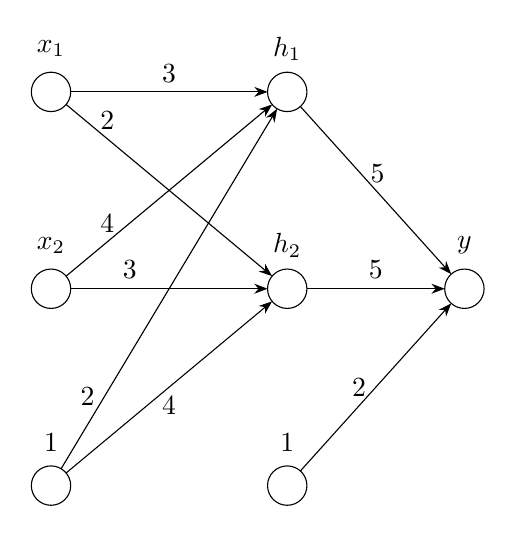
\begin{tikzpicture}
      \draw (0, 2.5) circle (0.25cm);
      \node at (0, 3.05) { $x_1$ };
      \draw (0, 0) circle (0.25cm);
      \node at (0, 0.55) { $x_2$ };
      \draw (0, -2.5) circle (0.25cm);
      \node at (0, -1.95) { $1$ };
      \draw (3, 2.5) circle (0.25cm);
      \node at (3, 3.05) { $h_1$ };
      \draw (3, 0) circle (0.25cm);
      \node at (3, 0.55) { $h_2$ };
      \draw (3, -2.5) circle (0.25cm);
      \node at (3, -1.95) { $1$ };
      \draw (5.25, 0) circle (0.25cm);
      \node at (5.25, 0.55) { $y$ };
      \draw[->] (0.25, 2.5) to (2.75, 2.5);
      \draw[->] (0.19205531989934396, 2.33995390008388) to (2.8079446801006562, 0.16004609991611995);
      \draw[->] (0.19205531989934396, 0.16004609991611995) to (2.8079446801006562, 2.33995390008388);
      \draw[->] (0.25, -1.5308084989341915e-17) to (2.75, 1.5308084989341915e-17);
      \draw[->] (0.12862393885688164, -2.285626768571864) to (2.8713760611431183, 2.285626768571864);
      \draw[->] (0.19205531989934396, -2.33995390008388) to (2.8079446801006562, -0.16004609991611995);
      \draw[->] (3.1672411829056126, 2.3141764634382085) to (5.082758817094388, 0.18582353656179157);
      \draw[->] (3.25, -1.5308084989341915e-17) to (5.0, 1.5308084989341915e-17);
      \draw[->] (3.1672411829056126, -2.3141764634382085) to (5.082758817094388, -0.18582353656179157);
      \node[above] at (1.5, 2.5) { 3 };
      \node[above] at (0.7152331919396064, 1.903972340050328) { 2 };
      \node[above] at (0.7152331919396064, 0.5960276599496719) { 4 };
      \node[above] at (1.0, -6.1232339957367656e-18) { 3 };
      \node[left] at (0.677174363314129, -1.3713760611431185) { 2 };
      \node[below] at (1.5, -1.25) { 4 };
      \node[right] at (3.933448236581123, 1.4628352926876418) { 5 };
      \node[above] at (4.125, 0.0) { 5 };
      \node[left] at (4.125, -1.25) { 2 };
    \end{tikzpicture}
  \end{center}
  Note that we have a bias inbetween each layer. The first one has weights 2 and -4, and the second one 
  has weight -2. Thus for this network, the weight matrices are defined to be 
  \[
    W = 
    \begin{bmatrix}
      3 & 4 & 2 \\
      2 & 3 & 4 \\
    \end{bmatrix}
    \hspace{1cm}
    U = \begin{bmatrix}
      5 & 5 & 2 \\
    \end{bmatrix}
  \]
  allowing us to write $\vec{h} = r(W\vec{x})$ and $y = r(U\vec{h})$, 
  or more explicitly, for a given input $(x_0, x_1)$
  \begin{align}
    h_1 = r(3x_1 + 4x_2 + 2)\\
    h_2 = r(2x_1 + 3x_2 + 4)\\
    y = r(5h_1 + 5h_2 + 2)
  \end{align}
  which we can use to calculate the network.
  Below is a table of how this neural network currently computes the XOR values.
  \begin{center}
    \begin{tabular}{ |p{1.5cm}||p{3cm}|p{3cm}|p{3.5cm}|p{1.5cm}| }
      \hline
      $(x_0, x_1)$ & $h_0$ & $h_1$ & $y$ & target\\
      \hline
      $(1, 0)$ & $\sigma(1) = 0.731$ & $\sigma(-2) = 0.119$ & $\sigma(1.060) = 0.743$ & 1 \\
      \hline
      $(0, 0)$ & $\sigma(-2) = 0.119$ & $\sigma(-4) = 0.018$ & $\sigma(-1.495) = 0.183$  & 0\\
      \hline
      $(0, 1)$ & $\sigma(2) = 0.881$ & $\sigma(-1) = 0.269$ & $\sigma(1.060) = 0.743$ & 1 \\
      \hline
      $(1, 1)$ & $\sigma(5) = 0.993$ & $\sigma(1) = 0.731$ & $\sigma(-0.690) = 0.334$ & 0\\
      \hline
     \end{tabular}
     
  \end{center}
  Based on the above table, we can see that so far it's not performing that well, but after 
  all it is a first stab. This now begs the question: What does it 
  mean for a model to perform well, and how do we know when it is improving? The answer
  to this is to introduce a \textbf{cost function} which can give a measure of error. There are 
  many possible choices for a cost function, but for simplicity we will use the \textbf{least squares}
  cost function. If we have a dataset of target values $t_i$, and our model currently 
  approximates this data with a set of values $y_i$, then the measured loss is 
  \[
      L = \frac{1}{2}\sum_{i}(t_i - y_i)^2
  \] 
  In our case, since the output of our function is in $\mathbb{R}$, we have 
  $L = \frac{1}{2}(t - y)^2$. 

  The concept of a cost function now leads to the strategy of back propagation: simply change the 
  model's weights in such a way as to minimize the cost function.

  In the case of our model, we need to find out what direction, and how much, we should ``push'' each 
  value of our existing matices $U$ and $W$, so as to minimize the cost function. 
  In terms of calculus, this means we are interested in the quantities 
  \[
      \frac{dL}{du_i} \hspace{1cm} \frac{dL}{dw_{ij}}
  \]
  Once we obtain these quantities, we can update our weights after reviewing one training
  example via
  \begin{align}
    u'_i &= u_i - \frac{dL}{du_i} \\
    w'_{ij}  &= w_{ij} - \frac{dL}{dw_{ij}}
  \end{align}
  First, let us calculate how the loss is affected by the weights in the final layer (i.e. the 
  entries of the matrix $U$). Since $y = r(\sum_{k}u_{k}h_k)$, we have that 
  \[
    \frac{dL}{du_i} = \frac{dL}{dy}\frac{dy}{du_i}
  \]
  Observe that 
  \[
    \frac{dL}{dy} = -(t - y)
  \]
  and 
  \[
    \frac{dy}{du_i} 
    = r'\left(\sum_{k}u_{k}h_k\right) \cdot \frac{d}{du_i}\left(\sum_{k}u_{k}h_k\right)
    = r'\left(\sum_{k}u_{k}h_k\right) \cdot h_i
  \]
  If we write $s_y = \sum_{k}u_kh_k$ (i.e. the summation before applying the activation $r$ 
  which calculates the value of $y$) then we can write
  \[
    \frac{dL}{du_i}
    = 
    -(t - y)r'(s_y)h_i.
  \]
  Next, let us calculate how the loss is affected by weights in the first layer (i.e. the entries 
  of the matrix $W$). Once again we have 
  \[
    \frac{dL}{dw_{ij}} = \frac{dL}{dy}\frac{dy}{dw_{ij}} = \frac{dL}{dy}\frac{dy}{dh_{i}}
    \frac{dh_i}{dw_{ij}} 
  \]
  We already know $\frac{dL}{dy}$. Thus we calculate 
  \begin{align}
    \frac{dy}{dh_{i}}
    &= r'\left(\sum_{k}u_{k}h_k\right) \cdot \frac{d}{dh_i}\left(\sum_{k}u_{k}h_k\right)\\
    &= r'\left(\sum_{k}u_{k}h_k\right) \cdot u_i\\
    &= r'(s_{y})u_i
  \end{align}
  and since $h_i = r\left( \sum_{k}w_{ik}x_k \right)$ we have that 
  \begin{align}
    \frac{dh_i}{dw_{ij}} 
    &= r'\left(\sum_{k}w_{ik}x_i\right) \cdot \frac{d}{dw_{ij}} \left( \sum_{k}w_{ik}x_k \right) \\
    &= r'\left(\sum_{k}w_{ik}x_i\right) \cdot x_j 
  \end{align}
  If we write $s_{h_i} = \sum_{k}w_{ik}h_k$, then we can write
  \[
    \frac{dh_i}{dw_{ij}} 
    = r'(s_{h_i})x_i
  \]
  Combining all of our calculations, we then get that 
  \[
    \frac{dL}{dw_{ij}}= -(t - y) \cdot r'(s_y)u_i \cdot r'(s_{h_i})x_j
  \]
  If we define $\delta = -(t - y)r'(s_y)$, interpreting it as an error term,
  we obtain the following explicit weight update formulas.
  \begin{align}
    u_1' &= u_1 - \delta h_1\\
    u_2' &= u_2 - \delta h_2\\
    w_{11}' &= w_{11} - \delta u_1r'(s_{h_1})x_1\\
    w_{12}' &= w_{12} - \delta u_1r'(s_{h_1})x_2\\
    w_{21}' &= w_{21} - \delta u_2r'(s_{h_2})x_1\\
    w_{22}' &= w_{22} - \delta u_2r'(s_{h_2})x_2\\
  \end{align}
  Recall that the weights $u_3$ (in $U$) and $w_{13}$, $w_{23}$ (in $W$) 
  correspond to the bias parameters in our model. Their weight update formulas are much simpler, 
  since the value of their origin node is automatically fixed to 1.
  \begin{align}
    u_3' &= u_3 - \delta \\
    w_{13}' &= w_{13} - \delta u_1r'(s_{h_1})\\
    w_{23}' &= w_{23} - \delta u_2r'(s_{h_2})\\
  \end{align}

  This completes our description for how we update our model's weights given 
  one training example. In practice, however, we tend to have many training examples 
  $t_1, t_2, \dots, t_N$ that we can use to update our model. 
  There are three main approaches as to exactly how we can update our 
  model's weights using all of the training examples.
  \begin{itemize}
    \item \textbf{Stochastic Gradient Descent.} Update the model's weights after each training example $t_i$.
    \item\textbf{Batch Gradient Descent.} Update the model's weights after showing it every training example. 
    In this case, we could achieve this by collecting all of the gradients calculated from each 
    training example and then averaging them.
    \[
      w'_{ij}  = w_{ij} - \frac{1}{N} \sum_{t_k}\frac{dL(t_k)}{dw_{ij}}
    \]
    \item\textbf{Mini-Batch Gradient Descent.} Update the model's weights after showing it $n < N$ many training 
    examples; we'd call $n$ our \textbf{batch size}. 
    This can be thought of as a compromise between stochastic and batch gradient descent. 
  \end{itemize}
  These three methods trade off training speed and model accuracy. As mini-batch is a compromise 
  between speed and accuracy, it tends to be preferred in practice. In any case, 
  in practice we tend to train the model on the training set each time; each iteration is 
  called an \textbf{epoch}, and so a training procedure may undergo several epochs.
  Too few epochs will lead to poor accuracy, but too many epochs will leads to 
  poor generalization outside of the training set, a concept known as \textbf{overfitting}.

  For this example, if we perform batch gradient descent on the model we presented, using our 
  four training examples of the XOR function,
  training this for tens of thousands of epochs
  will allow us to converge on these model weighs 
  \begin{align}
    W = 
    \begin{bmatrix}
      1.52183263 & 1.55282077 & -1.55282077 \\
      1.0637993 & 1.0637993 & 0.39200322 \\
    \end{bmatrix}\\
    U = \begin{bmatrix}
      -1.31420497 & 0.94002694 & -0.36849359\\
    \end{bmatrix}
  \end{align}
  which successfully mimic the XOR function.

  
  \section{Backpropagation: More generally}
    At this point we have so far only dealt with neural networks that have at 
    most one hidden layer and only one output node. In general, neural networks can be designed 
    to have many hidden layers and many outputs nodes. We now present the backpropagation
    algorithm for deep neural networks that have arbitrarily many output nodes.

    First, we introduce some notation.
    Consider a neural network with $N$ layers (including the input and output layers).
    Let $h_i^{n}$ denote the $i$-th hidden node in the $n$-th layer (hence $1 < n \le N$).
    Let $w_{ij}^{(n)}$ denote the weight going from node 
    $h_j^{(n-1)}$ to $h_i^{(n)}$. We'll denote the 
    matrix made up of the weights $w_{ij}^{(n)}$ to be $W_n$.
    Below is a snapshot 
    of this specific part of the neural network.

    \begin{center}
      \begin{tikzpicture}
        \draw (0, 0) circle (0.25cm);
        \draw (4, 1) circle (0.25cm);
        \draw[->] (0.24253562503633297, 0.06063390625908324) to (3.757464374963667, 0.9393660937409167);
        \node at (2.0, 1.0) { $w^{(n)}_{ij}$ };
        \node at (0.3, 0.75) { $h^{(n - 1)}_{j}$ };
        \node at (4.3, 1.75) { $h^{(n)}_{i}$ };
        \node at (0, 1.5) { $\vdots$ };
        \node at (0, -1) { $\vdots$ };
        \node at (4, 2.5) { $\vdots$ };
        \node at (4, 0) { $\vdots$ };
    \end{tikzpicture}
    \end{center}
    Suppose we are given a dataset to train the weights of our neural network. 
    Then this means that, given a cost function $L$, we are interested in the quantity
    \[
      \frac{dL}{dw_{ij}^{(n)}} 
    \] 
    where $1 \le n \le N$ and $i$, $j$ vary as valid indices over the overall weight matrix 
    $W_n$. Then we have the following result for general backpropagation.

    \begin{theorem}[\textbf{Backpropagation}]
      Let $h_{k}^{\ell}$ denote the $k$-th hidden unit in layer $\ell$ where $n \le \ell \le N$.
      Then for the weight $w^{(n)}_{ij}$, we have the recurrence relation 
      \[
        \frac{dh_k^{\ell}}{dw^{(n)}_{ij}}
        =
        h_k^{(\ell)}(s)
        \cdot
        \sum_{t}w_{kt}\frac{dh^{(\ell-1)}_t}{dw^{(n)}_{ij}}.
      \]
      In the special case of when
      $\ell = n$, we have that
      \[
        \frac{dh_k^{n}}{dw^{(n)}_{ij}} = 0
        \hspace{1cm} \text{if $k \ne i$, otherwise} \hspace{1cm} \frac{dh_i^{n}}{dw^{(n)}_{ij}} = h_i^n \cdot h_j^{(n -1)}
      \]
      We can then use to write a general update formula for all 
      weights
      \[
        w^{(n)}_{ij} = w^{(n)}_{ij} - \frac{dh_k^{n}}{dw^{(n)}_{ij}}
      \]
    \end{theorem}






\end{document}
